\documentclass[twoside]{book}

% Packages required by doxygen
\usepackage{fixltx2e}
\usepackage{calc}
\usepackage{doxygen}
\usepackage[export]{adjustbox} % also loads graphicx
\usepackage{graphicx}
\usepackage[utf8]{inputenc}
\usepackage{makeidx}
\usepackage{multicol}
\usepackage{multirow}
\PassOptionsToPackage{warn}{textcomp}
\usepackage{textcomp}
\usepackage[nointegrals]{wasysym}
\usepackage[table]{xcolor}

% Font selection
\usepackage[T1]{fontenc}
\usepackage[scaled=.90]{helvet}
\usepackage{courier}
\usepackage{amssymb}
\usepackage{sectsty}
\renewcommand{\familydefault}{\sfdefault}
\allsectionsfont{%
  \fontseries{bc}\selectfont%
  \color{darkgray}%
}
\renewcommand{\DoxyLabelFont}{%
  \fontseries{bc}\selectfont%
  \color{darkgray}%
}
\newcommand{\+}{\discretionary{\mbox{\scriptsize$\hookleftarrow$}}{}{}}

% Page & text layout
\usepackage{geometry}
\geometry{%
  a4paper,%
  top=2.5cm,%
  bottom=2.5cm,%
  left=2.5cm,%
  right=2.5cm%
}
\tolerance=750
\hfuzz=15pt
\hbadness=750
\setlength{\emergencystretch}{15pt}
\setlength{\parindent}{0cm}
\setlength{\parskip}{3ex plus 2ex minus 2ex}
\makeatletter
\renewcommand{\paragraph}{%
  \@startsection{paragraph}{4}{0ex}{-1.0ex}{1.0ex}{%
    \normalfont\normalsize\bfseries\SS@parafont%
  }%
}
\renewcommand{\subparagraph}{%
  \@startsection{subparagraph}{5}{0ex}{-1.0ex}{1.0ex}{%
    \normalfont\normalsize\bfseries\SS@subparafont%
  }%
}
\makeatother

% Headers & footers
\usepackage{fancyhdr}
\pagestyle{fancyplain}
\fancyhead[LE]{\fancyplain{}{\bfseries\thepage}}
\fancyhead[CE]{\fancyplain{}{}}
\fancyhead[RE]{\fancyplain{}{\bfseries\leftmark}}
\fancyhead[LO]{\fancyplain{}{\bfseries\rightmark}}
\fancyhead[CO]{\fancyplain{}{}}
\fancyhead[RO]{\fancyplain{}{\bfseries\thepage}}
\fancyfoot[LE]{\fancyplain{}{}}
\fancyfoot[CE]{\fancyplain{}{}}
\fancyfoot[RE]{\fancyplain{}{\bfseries\scriptsize Generated by Doxygen }}
\fancyfoot[LO]{\fancyplain{}{\bfseries\scriptsize Generated by Doxygen }}
\fancyfoot[CO]{\fancyplain{}{}}
\fancyfoot[RO]{\fancyplain{}{}}
\renewcommand{\footrulewidth}{0.4pt}
\renewcommand{\chaptermark}[1]{%
  \markboth{#1}{}%
}
\renewcommand{\sectionmark}[1]{%
  \markright{\thesection\ #1}%
}

% Indices & bibliography
\usepackage{natbib}
\usepackage[titles]{tocloft}
\setcounter{tocdepth}{3}
\setcounter{secnumdepth}{5}
\makeindex

% Hyperlinks (required, but should be loaded last)
\usepackage{ifpdf}
\ifpdf
  \usepackage[pdftex,pagebackref=true]{hyperref}
\else
  \usepackage[ps2pdf,pagebackref=true]{hyperref}
\fi
\hypersetup{%
  colorlinks=true,%
  linkcolor=blue,%
  citecolor=blue,%
  unicode%
}

% Custom commands
\newcommand{\clearemptydoublepage}{%
  \newpage{\pagestyle{empty}\cleardoublepage}%
}

\usepackage{caption}
\captionsetup{labelsep=space,justification=centering,font={bf},singlelinecheck=off,skip=4pt,position=top}

%===== C O N T E N T S =====

\begin{document}

% Titlepage & ToC
\hypersetup{pageanchor=false,
             bookmarksnumbered=true,
             pdfencoding=unicode
            }
\pagenumbering{roman}
\begin{titlepage}
\vspace*{7cm}
\begin{center}%
{\Large My Project }\\
\vspace*{1cm}
{\large Generated by Doxygen 1.8.11}\\
\end{center}
\end{titlepage}
\clearemptydoublepage
\tableofcontents
\clearemptydoublepage
\pagenumbering{arabic}
\hypersetup{pageanchor=true}

%--- Begin generated contents ---
\chapter{Data Science with C++ exercise}
\label{md_README}
\hypertarget{md_README}{}
Simple data science exercise demonstrating the use of these features\+:


\begin{DoxyItemize}
\item reading, writing, and parsing data
\item header+source files
\item O\+OP\+: inheritance, virtual methods, abstract base class, constructor+destructor, static variable+method (T\+O\+DO), polymorphism (T\+O\+DO)
\item data structures\+: struct, class, unordered map, vector
\item pointers, references (T\+O\+DO)
\item S\+TL, Boost
\item passing by reference/by value
\item dynamic memory allocation (T\+O\+DO)
\item C++11, C++14 features
\item templates (T\+O\+DO)
\item python like string formatting (with Boost Format)
\item printing in color
\item documentation
\item testing (with Google Test)
\item C\+LI arguments (T\+O\+DO)
\item make (T\+O\+DO)
\item include guards (via \#pragma once)
\item macros
\item namespaces (T\+O\+DO)
\item exceptions (T\+O\+DO)
\item regexes
\item plotting (T\+O\+DO)
\item external library (T\+O\+DO)
\item declaration vs definition
\item measing elapsed time
\end{DoxyItemize}

\# Setup 
\begin{DoxyCode}
1 # setup C++
2 sudo apt-get install g++
3 
4 # install boost
5 sudo apt-get install libboost-all-dev
6 
7 # install doxygen
8 sudo apt-get install doxygen
9 sudo apt-get install graphviz
10 
11 # generate a project-specific doxygen configuration file
12 doxygen -g parsing-exercise.conf
13 
14 # install astyle c++ prettyfier
15 download https://sourceforge.net/projects/astyle/files/latest/download?source=files
16 cd astyle/build/gcc
17 make
18 
19 # install code correctness recommender
20 sudo pip install --upgrade cppclean
21 
22 # install google test
23 sudo apt-get install libgtest-dev
24 sudo apt-get install cmake # install cmake
25 cd /usr/src/gtest
26 sudo cmake CMakeLists.txt
27 sudo make
28 # copy or symlink libgtest.a and libgtest\_main.a to your /usr/lib folder
29 sudo cp *.a /usr/lib
30 
31 # make run.sh executable
32 chmod +x run.sh
33 
34 # run
35 ./run.sh
\end{DoxyCode}


\section*{T\+O\+DO}


\begin{DoxyItemize}
\item better naming
\item better optimization
\item add tests
\item more comments
\item use typedefs
\item use initializers whenever you can
\item better project structure
\item make plot
\item add external library
\item write blog post
\item improve Boost formatting 
\end{DoxyItemize}
\chapter{Hierarchical Index}
\section{Class Hierarchy}
This inheritance list is sorted roughly, but not completely, alphabetically\+:\begin{DoxyCompactList}
\item \contentsline{section}{Data}{\pageref{classData}}{}
\begin{DoxyCompactList}
\item \contentsline{section}{Temperature\+Data}{\pageref{classTemperatureData}}{}
\end{DoxyCompactList}
\item \contentsline{section}{Record}{\pageref{structRecord}}{}
\end{DoxyCompactList}

\chapter{Class Index}
\section{Class List}
Here are the classes, structs, unions and interfaces with brief descriptions\+:\begin{DoxyCompactList}
\item\contentsline{section}{\hyperlink{classData}{Data} }{\pageref{classData}}{}
\item\contentsline{section}{\hyperlink{structRecord}{Record} }{\pageref{structRecord}}{}
\item\contentsline{section}{\hyperlink{classTemperatureData}{Temperature\+Data} }{\pageref{classTemperatureData}}{}
\end{DoxyCompactList}

\chapter{Class Documentation}
\hypertarget{classData}{}\section{Data Class Reference}
\label{classData}\index{Data@{Data}}


Inheritance diagram for Data\+:\nopagebreak
\begin{figure}[H]
\begin{center}
\leavevmode
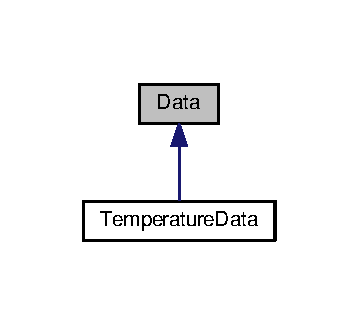
\includegraphics[width=172pt]{classData__inherit__graph}
\end{center}
\end{figure}
\subsection*{Public Member Functions}
\begin{DoxyCompactItemize}
\item 
{\bfseries Data} (std\+::string)\hypertarget{classData_a619cb123144821ee3cc9082a5e5e468d}{}\label{classData_a619cb123144821ee3cc9082a5e5e468d}

\item 
void {\bfseries print} ()\hypertarget{classData_a779ce878d01483220b49ad9e513d7366}{}\label{classData_a779ce878d01483220b49ad9e513d7366}

\item 
virtual void {\bfseries read} ()=0\hypertarget{classData_a16a784e96cd5e92785a0c4f2824284c7}{}\label{classData_a16a784e96cd5e92785a0c4f2824284c7}

\item 
virtual void {\bfseries save} (std\+::string, std\+::string sep=\char`\"{};\char`\"{})=0\hypertarget{classData_abfbd034f17ac92ce1fbad5f148abb80c}{}\label{classData_abfbd034f17ac92ce1fbad5f148abb80c}

\end{DoxyCompactItemize}
\subsection*{Protected Attributes}
\begin{DoxyCompactItemize}
\item 
std\+::string {\bfseries filename}\hypertarget{classData_a2cbdf542620c5f62b3e504ea2cecffd0}{}\label{classData_a2cbdf542620c5f62b3e504ea2cecffd0}

\item 
std\+::vector$<$ \hyperlink{structRecord}{Record} $>$ {\bfseries records}\hypertarget{classData_ab886b83cfa461cc7def5c0e8ba870d7c}{}\label{classData_ab886b83cfa461cc7def5c0e8ba870d7c}

\end{DoxyCompactItemize}


The documentation for this class was generated from the following files\+:\begin{DoxyCompactItemize}
\item 
temperature.\+h\item 
temperature.\+cpp\end{DoxyCompactItemize}

\hypertarget{structRecord}{}\section{Record Struct Reference}
\label{structRecord}\index{Record@{Record}}
\subsection*{Public Attributes}
\begin{DoxyCompactItemize}
\item 
std\+::string {\bfseries station}\hypertarget{structRecord_a594772e9772b63fa5897512bc618bf58}{}\label{structRecord_a594772e9772b63fa5897512bc618bf58}

\item 
double {\bfseries temperature}\hypertarget{structRecord_a04ffa52863d86812a456d566b10266e1}{}\label{structRecord_a04ffa52863d86812a456d566b10266e1}

\end{DoxyCompactItemize}


The documentation for this struct was generated from the following file\+:\begin{DoxyCompactItemize}
\item 
temperature.\+h\end{DoxyCompactItemize}

\hypertarget{classTemperatureData}{}\section{Temperature\+Data Class Reference}
\label{classTemperatureData}\index{Temperature\+Data@{Temperature\+Data}}


Inheritance diagram for Temperature\+Data\+:\nopagebreak
\begin{figure}[H]
\begin{center}
\leavevmode
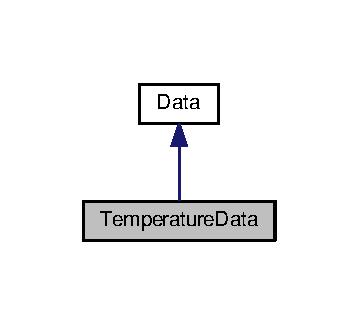
\includegraphics[width=172pt]{classTemperatureData__inherit__graph}
\end{center}
\end{figure}


Collaboration diagram for Temperature\+Data\+:\nopagebreak
\begin{figure}[H]
\begin{center}
\leavevmode
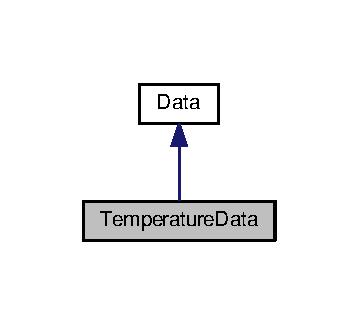
\includegraphics[width=172pt]{classTemperatureData__coll__graph}
\end{center}
\end{figure}
\subsection*{Public Member Functions}
\begin{DoxyCompactItemize}
\item 
void {\bfseries read} ()\hypertarget{classTemperatureData_ac481b4de9ca185ac241f991d954c5794}{}\label{classTemperatureData_ac481b4de9ca185ac241f991d954c5794}

\item 
records\+\_\+by\+\_\+station {\bfseries to\+\_\+map} () const \hypertarget{classTemperatureData_a3c6e7348c016f1521a1516f6d90387f8}{}\label{classTemperatureData_a3c6e7348c016f1521a1516f6d90387f8}

\item 
void {\bfseries save} (std\+::string, std\+::string sep=\char`\"{};\char`\"{}) const \hypertarget{classTemperatureData_a5360404200e4daa1643dcca45badae28}{}\label{classTemperatureData_a5360404200e4daa1643dcca45badae28}

\end{DoxyCompactItemize}
\subsection*{Additional Inherited Members}


The documentation for this class was generated from the following files\+:\begin{DoxyCompactItemize}
\item 
temperature.\+h\item 
temperature.\+cpp\end{DoxyCompactItemize}

%--- End generated contents ---

% Index
\backmatter
\newpage
\phantomsection
\clearemptydoublepage
\addcontentsline{toc}{chapter}{Index}
\printindex

\end{document}
